\section[Intro]{Introduction}

%%%%%%%%%%%%%%%%%%%%%%%%%%%%%%%%%%%%%%%%%%%%%%%%%%%%%%%%%%%%%%%%%%%%%%%%%%%%%%%%%%
\begin{frame}[fragile]\frametitle{}
\begin{center}
{\Large Introduction}
\end{center}
\end{frame}

%%%%%%%%%%%%%%%%%%%%%%%%%%%%%%%%%%%%%%%%%%%%%%%%%%%%%%%%%%%%%%%%%%%%%%%%%%%%%%%%%%
\begin{frame}[fragile]\frametitle{Why 'Go' after Reinforcement Learning?}

\begin{center}
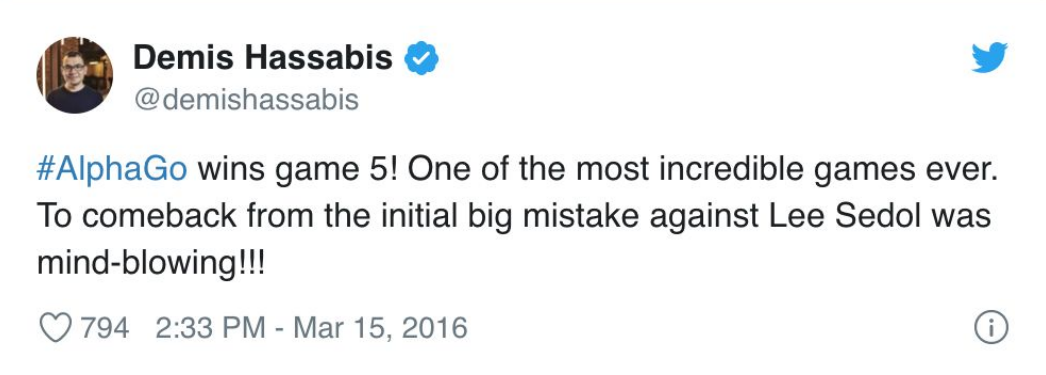
\includegraphics[width=0.5\linewidth,keepaspectratio]{rl12}

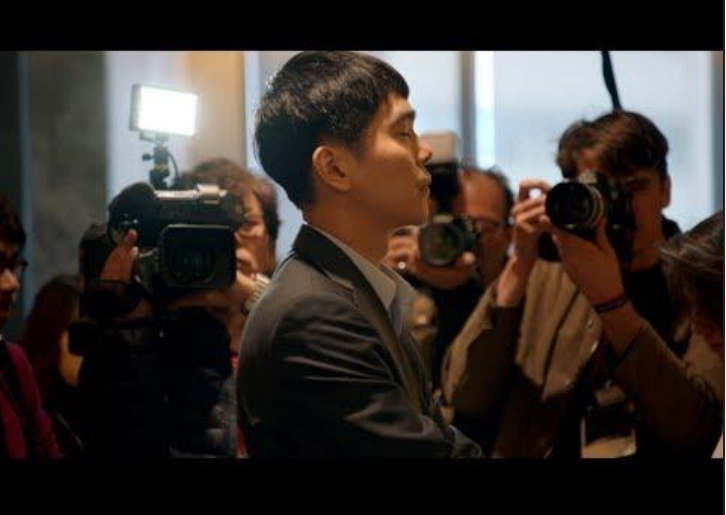
\includegraphics[width=0.5\linewidth,keepaspectratio]{rl13}

Alpha Go (4) vs Lee Sedol (1)
\end{center}

\end{frame}

%%%%%%%%%%%%%%%%%%%%%%%%%%%%%%%%%%%%%%%%%%%%%%%%%%%%%%%%%%%%%%%%%%%%%%%%%%%%%%%%%%
\begin{frame}[fragile]\frametitle{Brief History}

\begin{center}
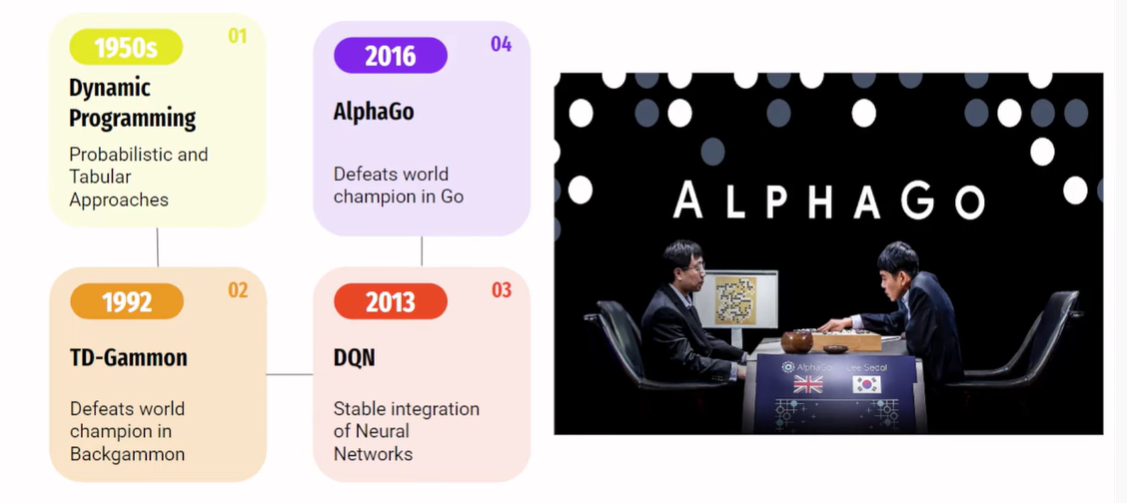
\includegraphics[width=\linewidth,keepaspectratio]{rl17}
\end{center}

{\tiny (Ref: But what is Reinforcement Learning? | Reinforcement Learning Part-1 - Rajtilak Pal (M. Tech in AI, IIT Ropar))}
\end{frame}


%%%%%%%%%%%%%%%%%%%%%%%%%%%%%%%%%%%%%%%%%%%%%%%%%%%%%%%%%%%%%%%%%%%%%%%%%%%%%%%%%%
\begin{frame}[fragile]\frametitle{What is Reinforcement Learning?}
Reinforcement Learning(RL) is a type of machine learning technique that enables an agent to learn in an interactive environment by trial and error using feedback from its own actions and experiences.

\begin{center}
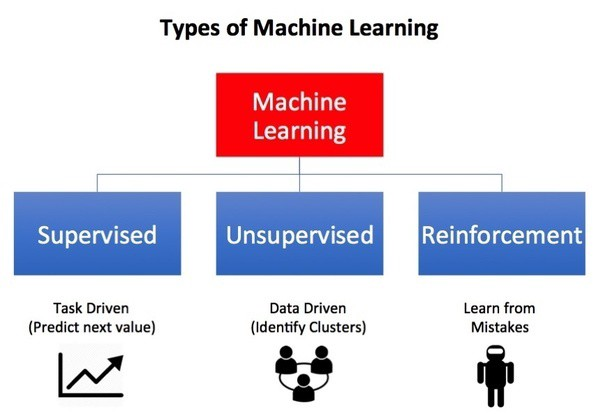
\includegraphics[width=0.6\linewidth,keepaspectratio]{rl9}
\end{center}


\end{frame}

%%%%%%%%%%%%%%%%%%%%%%%%%%%%%%%%%%%%%%%%%%%%%%%%%%%%%%%%%%%%%%%%%%%%%%%%%%%%%%%%%%
\begin{frame}[fragile]\frametitle{What is Reinforcement Learning?}

\begin{itemize}
\item Rule-based System: input is given, you write rules/logic to generate expected output
\item Machine Learning: Input and output, both are given, logic/model is fitted to the data
	\begin{itemize}
	\item Tabular: all rows are independent, can be processed in any order, output is at the end
	\item Sequential: input is in form of sequence and output is at the end, e.g., Sentiment analysis
	\end{itemize}
\item Reinforcement Learning: 
	\begin{itemize}
	\item Sequential decision making 
	\item Problem setup as agent in unknown environment. 
	\item Goal: select action to maximize a future cumulative reward
	\item Machine Learning learns the data, whereas RL learns the Goal
	\end{itemize}
\end{itemize}

\end{frame}

%%%%%%%%%%%%%%%%%%%%%%%%%%%%%%%%%%%%%%%%%%%%%%%%%%%%%%%%%%%
\begin{frame}[fragile]\frametitle{Differences}
\begin{center}
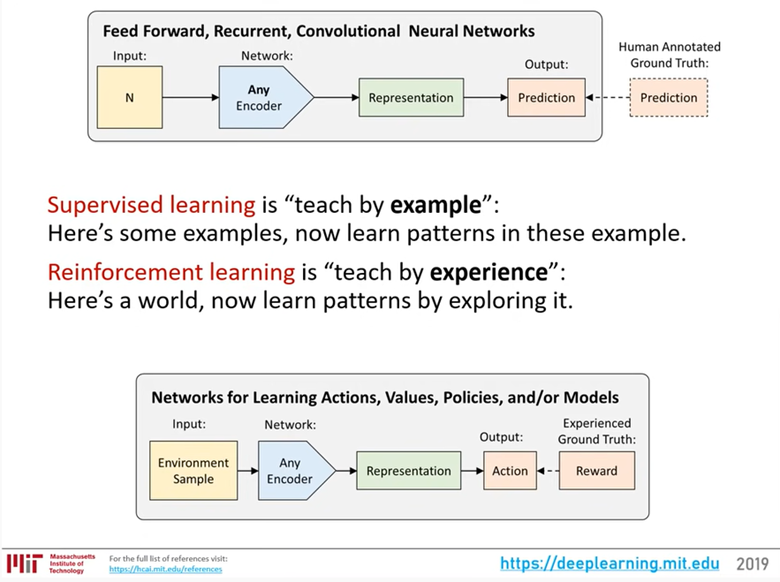
\includegraphics[width=0.9\linewidth,keepaspectratio]{rl25}
\end{center}
\end{frame}

%%%%%%%%%%%%%%%%%%%%%%%%%%%%%%%%%%%%%%%%%%%%%%%%%%%%%%%%%%%%%%%%%%%%%%%%%%%%%%%%%%
\begin{frame}[fragile]\frametitle{Comparison with ML}

\begin{itemize}
\item If you have labeled data; go for Supervised ML || In $f(X) = y$; given $X$ and $y$,  find $f$.
\item If you have no labels but data; go for Unsupervised ML || Given $X$ and no $y$,  find groups within $X$
\item If you have no data; go for Reinforcement Learning || Given no ready pairs of $X$ and $y$ but a notion of reward $z$, find $f$; $X$ is states, $y$ is action, in RL we are finding policy ie $f(X)$ using a helper quantity $z$.
\end{itemize}


\end{frame}


%%%%%%%%%%%%%%%%%%%%%%%%%%%%%%%%%%%%%%%%%%%%%%%%%%%%%%%%%%%%%%%%%%%%%%%%%%%%%%%%%%
\begin{frame}[fragile]\frametitle{Comparison with Humans}

Humans appear to learn to walk through ``very few examples'' of trial and error. How is an open question…Possible answers?:
\begin{itemize}
\item Hardware: 230 million years of bipedal movement data.
\item Imitation Learning: Observation of other humans walking.
\item Algorithms: Better than back-propagation and stochastic gradient descent
\end{itemize}


\end{frame}



%%%%%%%%%%%%%%%%%%%%%%%%%%%%%%%%%%%%%%%%%%%%%%%%%%%%%%%%%%%%%%%%%%%%%%%%%%%%%%%%%%
\begin{frame}[fragile]\frametitle{Comparison}

Advantages:
\begin{itemize}
\item Less labeled data, almost like bootstrapping
\item Structurally suitable for reward/penalty-based problems
\item As less data, less bias, ethically batter
\end{itemize}

Disadvantages:
\begin{itemize}
\item Take very long to converge, huge compute requirements
\item Does not generalize well. Small change in environment fails it
\end{itemize}

\end{frame}


%%%%%%%%%%%%%%%%%%%%%%%%%%%%%%%%%%%%%%%%%%%%%%%%%%%%%%%%%%%%%%%%%%%%%%%%%%%%%%%%%%
\begin{frame}[fragile]\frametitle{High Level}

\begin{itemize}
\item   Goal: Select actions to maximize expected cumulative future reward. (The Returns are $Expected$ as many a times they can be stochastic and not deterministic)
\item   Requires: Balancing short term and long term rewards, Strategy to maximize rewards
\item   Example: Web Advertising
\end{itemize}


\end{frame}



%%%%%%%%%%%%%%%%%%%%%%%%%%%%%%%%%%%%%%%%%%%%%%%%%%%%%%%%%%%%%%%%%%%%%%%%%%%%%%%%%%
\begin{frame}[fragile]\frametitle{Definitions}
\begin{itemize}
\item Reinforcement learning, a type of machine learning, in which agents take actions in an environment aimed at maximizing their cumulative rewards – NVIDIA

\item Reinforcement learning (RL) is based on rewarding desired behaviors or punishing undesired ones. Instead of one input producing one output, the algorithm produces a variety of outputs and is trained to select the right one based on certain variables – Gartner

\item It is a type of machine learning technique where a computer agent learns to perform a task through repeated trial and error interactions with a dynamic environment. This learning approach enables the agent to make a series of decisions that maximize a reward metric for the task without human intervention and without being explicitly programmed to achieve the task – Mathworks
\end{itemize}
\end{frame}

%%%%%%%%%%%%%%%%%%%%%%%%%%%%%%%%%%%%%%%%%%%%%%%%%%%%%%%%%%%%%%%%%%%%%%%%%%%%%%%%%%
\begin{frame}[fragile]\frametitle{Essentially}
\begin{itemize}
\item Interactive Learning within an Environment, like a student and a teacher
\item Learning by trial and error, with adaptive control
\item Goal is to build a policy-recipe for maximizing reward.
\item Agent interacts with an Environment, with a feedback loop
\item Agent finds optimum policy-strategy-recipe for making decision for better long term rewards.
\end{itemize}
\end{frame}

%%%%%%%%%%%%%%%%%%%%%%%%%%%%%%%%%%%%%%%%%%%%%%%%%%%%%%%%%%%%%%%%%%%%%%%%%%%%%%%%%%
\begin{frame}[fragile]\frametitle{ML vs RL}

\begin{itemize}
\item RL is part of ML
\item Supervised ML learns the training data, tries to generalize it. But needs large amounts of labeled data.
\item Unsupervised ML also needs data, but unlabeled. Tries to find groups based on similarity.
\item RL does not need labeled data. It needs formulation for rewards and an Environment that can be poked. Maximizing Reward is the goal. Does not try to find pattern in the data (well, data is not there anyway).
\end{itemize}

\begin{center}
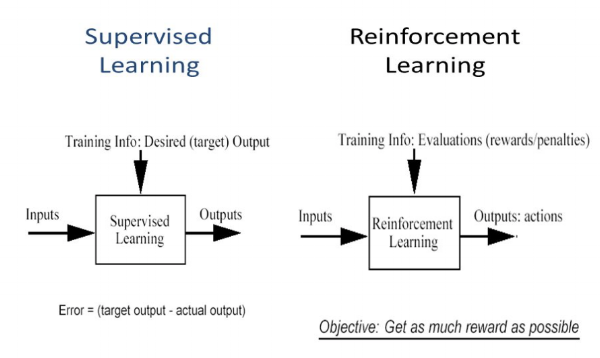
\includegraphics[width=0.5\linewidth,keepaspectratio]{rl7}
\end{center}

{\tiny (Ref: Introduction to Reinforcement Learning for Beginners - Analytics Vidhya)} 

\end{frame}

%%%%%%%%%%%%%%%%%%%%%%%%%%%%%%%%%%%%%%%%%%%%%%%%%%%%%%%%%%%%%%%%%%%%%%%%%%%%%%%%%%
\begin{frame}[fragile]\frametitle{Characteristics}
\begin{itemize}
\item No supervision, only a real value or reward signal
\item Decision making is sequential
\item Time plays a major role in reinforcement problems
\item Feedback isn’t prompt but delayed
\item The following data it receives is determined by the agent’s actions
\end{itemize}
\end{frame}


%%%%%%%%%%%%%%%%%%%%%%%%%%%%%%%%%%%%%%%%%%%%%%%%%%%%%%%%%%%%%%%%%%%%%%%%%%%%%%%%%%
\begin{frame}[fragile]\frametitle{Approaches}

\begin{center}
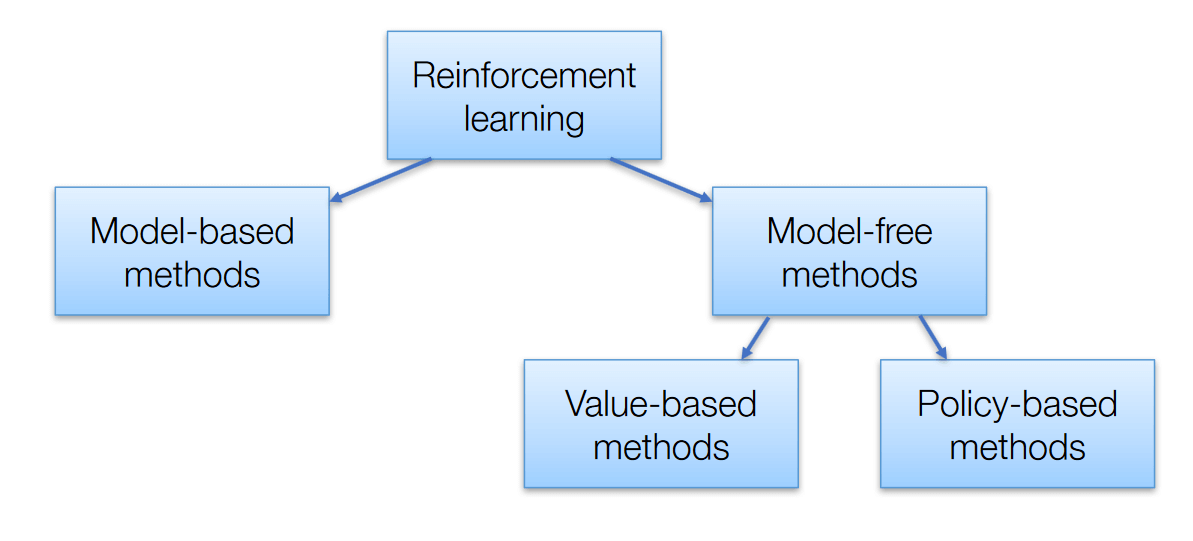
\includegraphics[width=0.5\linewidth,keepaspectratio]{rl8}

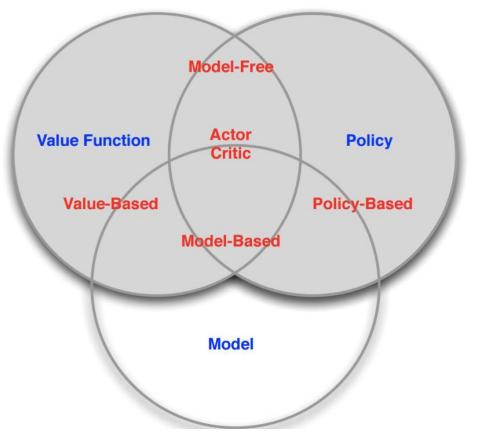
\includegraphics[width=0.4\linewidth,keepaspectratio]{rl15}

\end{center}

{\tiny (Ref: Reinforcement Learning Algorithms – AISummer)} 


\end{frame}


%%%%%%%%%%%%%%%%%%%%%%%%%%%%%%%%%%%%%%%%%%%%%%%%%%%%%%%%%%%%%%%%%%%%%%%%%%%%%%%%%%
\begin{frame}[fragile]\frametitle{Approaches}

\begin{itemize}
\item Value-Based – The main goal of this method is to maximize a value function. Here, an agent through a policy expects a long-term return of the current states.

\item Policy-Based – In policy-based, you enable to come up with a strategy that helps to gain maximum rewards in the future through possible actions performed in each state. Two types of policy-based methods are deterministic and stochastic.

\item Model-Based – In this method, we need to create a virtual model for the agent to help in learning to perform in each specific environment
\end{itemize}

\end{frame}

%%%%%%%%%%%%%%%%%%%%%%%%%%%%%%%%%%%%%%%%%%%%%%%%%%%%%%%%%%%%%%%%%%%%%%%%%%%%%%%%%%
\begin{frame}[fragile]\frametitle{Algorithms}

\begin{center}
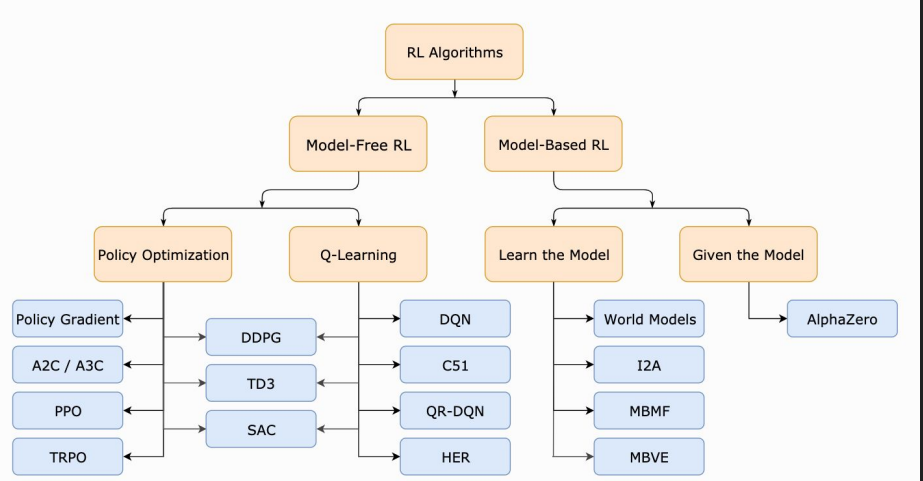
\includegraphics[width=\linewidth,keepaspectratio]{rl16}
\end{center}

\end{frame}

% %%%%%%%%%%%%%%%%%%%%%%%%%%%%%%%%%%%%%%%%%%%%%%%%%%%%%%%%%%%%%%%%%%%%%%%%%%%%%%%%%%
% \begin{frame}[fragile]\frametitle{Algorithms}
% \begin{center}
% 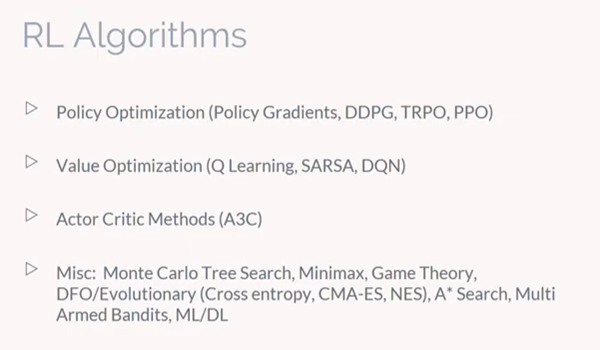
\includegraphics[width=\linewidth,keepaspectratio]{rl30}
% \end{center}

% {\tiny (Ref: Deep Learning - MIT 2019)}

% \end{frame}


%%%%%%%%%%%%%%%%%%%%%%%%%%%%%%%%%%%%%%%%%%%%%%%%%%%%%%%%%%%%%%%%%%%%%%%%%%%%%%%%%%
\begin{frame}[fragile]\frametitle{Algorithms}

\begin{itemize}
\item Q-learning and SARSA (State-Action-Reward-State-Action): commonly used model-free RL algorithms. 
\item Differ in terms of their exploration strategies while their exploitation strategies are similar. 
\item While Q-learning is an off-policy method in which the agent learns the value based on action a* derived from the another policy, SARSA is an on-policy method where it learns the value based on its current action a derived from its current policy.
\item Both lack generality as they do not have the ability to estimates values for unseen states.
\item Solution:  Deep Q-Networks(DQNs) which use Neural Networks to estimate Q-values. But DQNs can only handle discrete, low-dimensional action spaces.
\item Deep Deterministic Policy Gradient(DDPG) is a model-free, off-policy, actor-critic algorithm that tackles this problem by learning policies in high dimensional, continuous action spaces. The figure below is a representation of actor-critic architecture.
\end{itemize}




\end{frame}

%%%%%%%%%%%%%%%%%%%%%%%%%%%%%%%%%%%%%%%%%%%%%%%%%%%%%%%%%%%%%%%%%%%%%%%%%%%%%%%%%%
\begin{frame}[fragile]\frametitle{Implementation platforms}

\begin{itemize}
\item RLib - Ray Berkley
\item Tf Agents - Google
\item Open AI Gym
\item Project Malmo - Microsoft
\item DeepMind Lab
\end{itemize}

\end{frame}

%%%%%%%%%%%%%%%%%%%%%%%%%%%%%%%%%%%%%%%%%%%%%%%%%%%%%%%%%%%%%%%%%%%%%%%%%%%%%%%%%%
\begin{frame}[fragile]\frametitle{Applications}

\begin{itemize}
\item Robotics for Industrial Automation
\item Text summarization engines, dialog agents (text, speech), game-plays
\item Autonomous Self Driving Cars
\item Machine Learning and Data Processing
\item Training system which would issue custom instructions and materials with respect to the requirements of students
\item AI Toolkits, Manufacturing, Automotive, Health-care, and Bots
\item Aircraft Control and Robot Motion Control
\item Building artificial intelligence for computer games
\end{itemize}

\end{frame}

\section[MDP]{Markov Decision Process}

%%%%%%%%%%%%%%%%%%%%%%%%%%%%%%%%%%%%%%%%%%%%%%%%%%%%%%%%%%%%%%%%%%%%%%%%%%%%%%%%%%
\begin{frame}[fragile]\frametitle{}
\begin{center}
{\Large Markov Decision Process}
\end{center}
\end{frame}



%%%%%%%%%%%%%%%%%%%%%%%%%%%%%%%%%%%%%%%%%%%%%%%%%%%%%%%%%%%
\begin{frame}[fragile]\frametitle{Formally}
\begin{center}
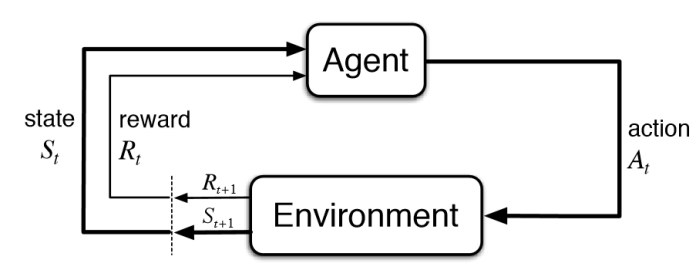
\includegraphics[width=0.6\linewidth,keepaspectratio]{rl1}
\end{center}

\begin{itemize}
\item Environment has States
\item Agent has a Policy with which it decides the Action.
\end{itemize}
\end{frame}

%%%%%%%%%%%%%%%%%%%%%%%%%%%%%%%%%%%%%%%%%%%%%%%%%%%%%%%%%%%%%%%%%%%%%%%%%%%%%%%%%%
\begin{frame}[fragile]\frametitle{The Whole Process}

\begin{center}
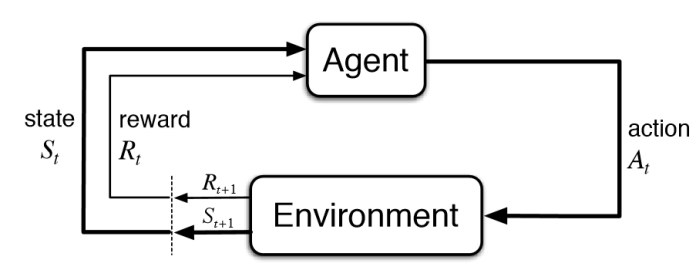
\includegraphics[width=0.6\linewidth,keepaspectratio]{rl1}
\end{center}

\begin{itemize}
\item Environment is like a black box, it is poked with Action
\item Once an Action comes to the Environment, it changes its State and that changed State is communicated back to the Agent.
\item Along with that, the Environment also communicates if any Reward/Penalty was acquired or not.
\item Just by poking multiple times, the Agent learns (thats Machine Learning) and builds such a Policy-Strategy-recipes, that the next Action proposed will get a Reward rather than Penalty.
\end{itemize}
\end{frame}


%%%%%%%%%%%%%%%%%%%%%%%%%%%%%%%%%%%%%%%%%%%%%%%%%%%%%%%%%%%%%%%%%%%%%%%%%%%%%%%%%%
\begin{frame}[fragile]\frametitle{Approaches}
\begin{center}
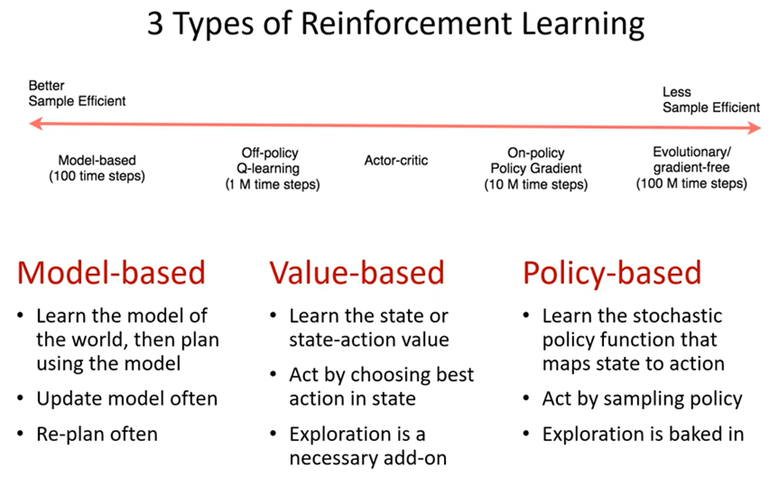
\includegraphics[width=0.9\linewidth,keepaspectratio]{rl26}
\end{center}

{\tiny (Ref: Deep Learning - MIT 2019)}

\end{frame}



%%%%%%%%%%%%%%%%%%%%%%%%%%%%%%%%%%%%%%%%%%%%%%%%%%%%%%%%%%%%%%%%%%%%%%%%%%%%%%%%%%
\begin{frame}[fragile]\frametitle{Types of sequential decision making}

\begin{columns}
\begin{column}{0.5\textwidth}

\begin{itemize}
\item Markov Decision Processes (MDPs and POMDPs)
	\begin{itemize}
	\item Agent’s state is dynamic
	\item Actions influence future observations
	\end{itemize}
\item Bandits
	\begin{itemize}
	\item Agent’s state is fixed
	\item Actions have no influence on next observations
	\end{itemize}
\end{itemize}

\end{column}
\begin{column}{0.5\textwidth}  %%<--- here

\begin{itemize}
\item Multi-arm bandits	
	\begin{itemize}
	\item Task: Choose repeatedly from one of n actions (play)
	\item Objective: optimize long term cumulative reward
	\end{itemize}
\item Contextual bandits	
	\begin{itemize}
	\item Context: extra information that can be used for making better decision when choosing amongst all actions
	\item Example, user history, preferences, etc
	\end{itemize}	
\end{itemize}

\end{column}
\end{columns}




\end{frame}


%%%%%%%%%%%%%%%%%%%%%%%%%%%%%%%%%%%%%%%%%%%%%%%%%%%%%%%%%%%%%%%%%%%%%%%%%%%%%%%%%%
\begin{frame}[fragile]\frametitle{Models}

\begin{itemize}
\item Markov Decision Process: MDP is a mathematical framework to describe an environment in RL and almost all RL problems can be formulated using MDPs. The outcome of deploying an action to a state doesn’t depend on previous actions or states but on current action and state.
\item Q Learning – it’s a value-based model free approach for supplying information to intimate which action an agent should perform. It revolves around the notion of updating Q values which shows the value of doing action A in state S.
\end{itemize}


\end{frame}


%%%%%%%%%%%%%%%%%%%%%%%%%%%%%%%%%%%%%%%%%%%%%%%%%%%%%%%%%%%%%%%%%%%%%%%%%%%%%%%%%%
\begin{frame}[fragile]\frametitle{Concepts}
\begin{center}
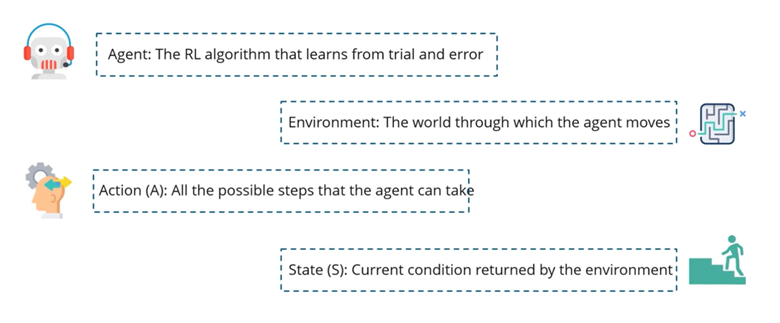
\includegraphics[width=0.6\linewidth,keepaspectratio]{rl31}

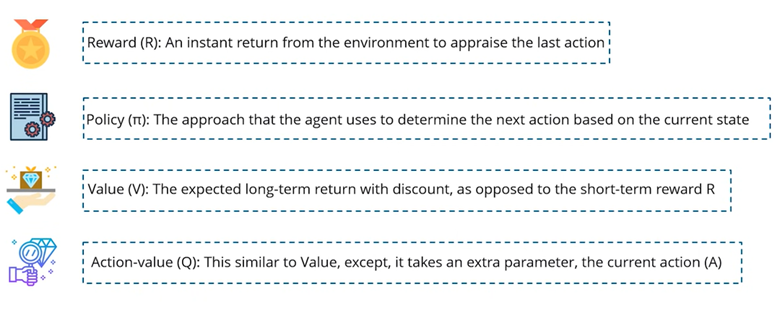
\includegraphics[width=0.6\linewidth,keepaspectratio]{rl32}

\end{center}

{\tiny (Ref: Reinforcement Learning Example Using Python - Edureka)}

\end{frame}

%%%%%%%%%%%%%%%%%%%%%%%%%%%%%%%%%%%%%%%%%%%%%%%%%%%%%%%%%%%%%%%%%%%%%%%%%%%%%%%%%%
\begin{frame}[fragile]\frametitle{Concepts}
\begin{center}
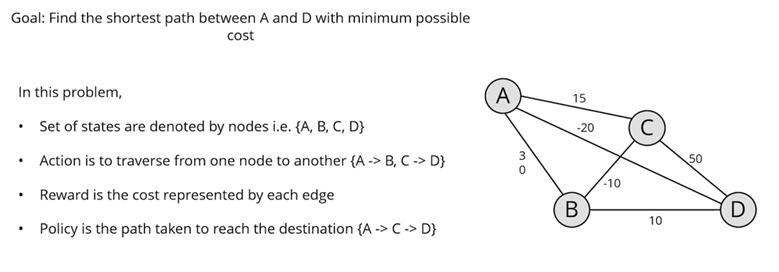
\includegraphics[width=0.9\linewidth,keepaspectratio]{rl33}

\end{center}

{\tiny (Ref: Reinforcement Learning Example Using Python - Edureka)}

\end{frame}


%%%%%%%%%%%%%%%%%%%%%%%%%%%%%%%%%%%%%%%%%%%%%%%%%%%%%%%%%%%%%%%%%%%%%%%%%%%%%%%%%%
\begin{frame}[fragile]\frametitle{MDP}

\begin{itemize}
\item MDP defines how an Agent takes sequential Actions from a State to State.
\item MDP formulation: $(S,A,R,\lambda)$, where,
	\begin{itemize}
	\item $S$ : State space
	\item $A$ : Action space
	\item $R$ : Reward function
	\item $\lambda$ : Discount factor
	\end{itemize}
\end{itemize}

\begin{center}
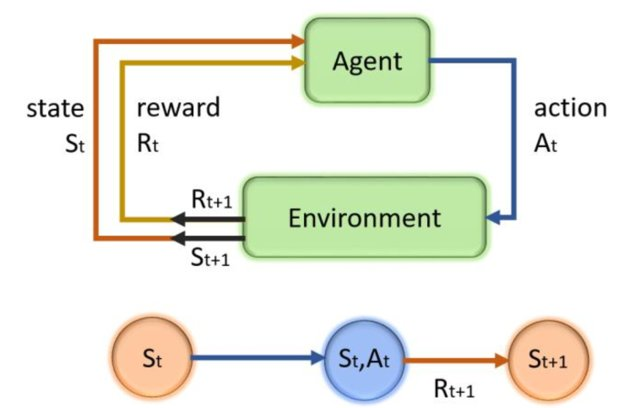
\includegraphics[width=0.6\linewidth,keepaspectratio]{rl2}
\end{center}

\end{frame}

%%%%%%%%%%%%%%%%%%%%%%%%%%%%%%%%%%%%%%%%%%%%%%%%%%%%%%%%%%%%%%%%%%%%%%%%%%%%%%%%%%
\begin{frame}[fragile]\frametitle{MDP}

\begin{center}
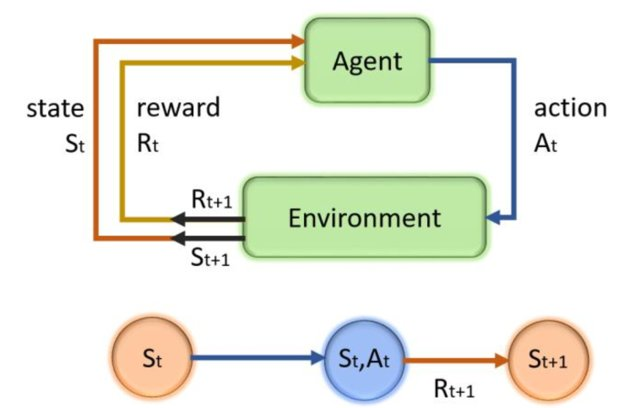
\includegraphics[width=0.6\linewidth,keepaspectratio]{rl2}
\end{center}

\begin{itemize}
\item Time steps $t = 0,1,2,3,\ldots$
\item At time step $t$, the Agent receives State, $S_t \in S$ and selects an Action $A_t \in A(S)$
\item One time step later $t+1$, the Agent receives Reward $R_{t+1} \in R$ and the Environment transitions to a new State $S_{t+1}$
\item Thus, MDP is a sequence : $S_0,A_0,R_1,S_1,A_1,R_2,S_2,A_2,R_3\ldots$
\end{itemize}

\end{frame}

%%%%%%%%%%%%%%%%%%%%%%%%%%%%%%%%%%%%%%%%%%%%%%%%%%%%%%%%%%%%%%%%%%%%%%%%%%%%%%%%%%
\begin{frame}[fragile]\frametitle{Expected Returns}

\begin{itemize}
\item Agents goal is to maximize Expected Returns
\item Returns is the sum of future rewards.
\item Goal $G_t= R_{t+1} + R_{t+2} + R_{t+3} + \ldots + R_n = \sum_{t=1}^{n}R_t$
\item Agent cares more about immediate rewards than the future ones. The Goal is updated as \ldots
\item Goal $G_t= R_{t+1} + \gamma R_{t+2} + \gamma^2 R_{t+3} + \ldots + \gamma^{n-1}R_n = \sum_{t=1}^{n}\gamma^{n-1}R_t$
\item At $\gamma = 0$ the Agent will be completely myopic. Looks at only immediate Reward.
\item At $\gamma = 1$ the Agent does not discount future Rewards but treats them equally.
\item $\gamma$ is typically between 0 and 1.

\end{itemize}

\end{frame}

%%%%%%%%%%%%%%%%%%%%%%%%%%%%%%%%%%%%%%%%%%%%%%%%%%%%%%%%%%%%%%%%%%%%%%%%%%%%%%%%%%
\begin{frame}[fragile]\frametitle{Observability}
When Observations are same as States (meaning, everything is fully visible, like in board games) the Environment is called as Fully Observable. If not, meaning, Observations occlude underlying real State, then truth is not fully known, thats Partially Observation Environment

\begin{center}
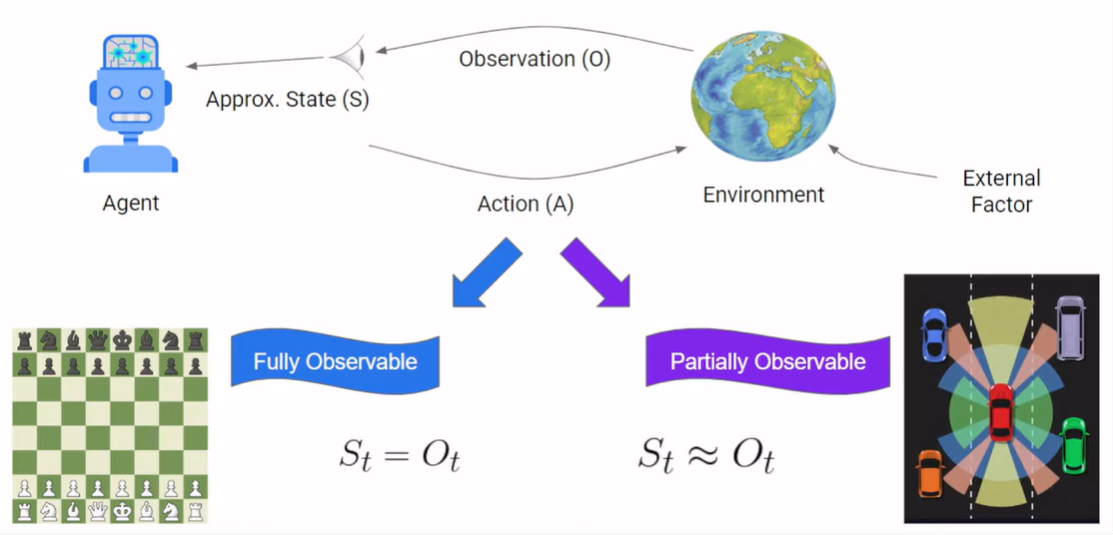
\includegraphics[width=\linewidth,keepaspectratio]{rl22}
\end{center}

{\tiny (Ref: But what is Reinforcement Learning? | Reinforcement Learning Part-1 - Rajtilak Pal (M. Tech in AI, IIT Ropar))}

\end{frame}

%%%%%%%%%%%%%%%%%%%%%%%%%%%%%%%%%%%%%%%%%%%%%%%%%%%%%%%%%%%%%%%%%%%%%%%%%%%%%%%%%%
\begin{frame}[fragile]\frametitle{Episodic vs Continuous}

Episodic:
\begin{itemize}
\item Interaction is naturally split into sequence, ie discrete events, eg. Table Tennis
\item Final steps is when point is scored (time of the reward)
\item Next episode begins Independently of how the previous was ended.
\end{itemize}

Continuous:
\begin{itemize}
\item Interaction is naturally smooth ie continuous flow, so no time steps as such.
\item Thus, Reward has to be function and at times even States have to be so.
\end{itemize}

\end{frame}



%%%%%%%%%%%%%%%%%%%%%%%%%%%%%%%%%%%%%%%%%%%%%%%%%%%%%%%%%%%%%%%%%%%%%%%%%%%%%%%%%%
\begin{frame}[fragile]\frametitle{Exploration vs Exploitation}

Challenges

\begin{itemize}
\item Deterministic/greedy policy won’t explore all actions
	\begin{itemize}
	\item Don’t know anything about the environment at the beginning
	\item Need to try all actions to find the optimal one
	\end{itemize}

\item $\epsilon$-greedy policy
	\begin{itemize}
	\item	With probability $1-\epsilon$ perform the optimal/greedy action, otherwise random action
	\item	Slowly move it towards greedy policy: $\epsilon \rightarrow 0$
	\end{itemize}
\item Agent can decide next Action based on, either
	\begin{itemize}
	\item Experiences so far (called Exploitation), or
	\item just random (called Exploration)
	\end{itemize}
\item Till enough experiences are built, Exploration is used. Also, it can give a random twist, which brings generation, and unexplored paths.
\item Full Exploitation: Greedy Agent
\item Full Exploration: Random
\item Need to find a balance and also when to use what.
\end{itemize}
\end{frame}


\section[Concepts]{Concepts}

%%%%%%%%%%%%%%%%%%%%%%%%%%%%%%%%%%%%%%%%%%%%%%%%%%%%%%%%%%%%%%%%%%%%%%%%%%%%%%%%%%
\begin{frame}[fragile]\frametitle{}
\begin{center}
{\Large Concepts}
\end{center}
\end{frame}


%%%%%%%%%%%%%%%%%%%%%%%%%%%%%%%%%%%%%%%%%%%%%%%%%%%%%%%%%%%%%%%%%%%%%%%%%%%%%%%%%%
\begin{frame}[fragile]\frametitle{Questions}

\begin{itemize}
\item What is the probability that an Agent will select as specific Action while being in some State?
\item How good the proposed Action is at the given State? as this 'goodness' decides the Reward.
\end{itemize}

\end{frame}

%%%%%%%%%%%%%%%%%%%%%%%%%%%%%%%%%%%%%%%%%%%%%%%%%%%%%%%%%%%%%%%%%%%%%%%%%%%%%%%%%%
\begin{frame}[fragile]\frametitle{Agent}

A system that is:

\begin{itemize}
\item situated in an environment
\item is capable of perceiving its environment,
\item is capable of acting in its environment
\item with the goal of satisfying its design objectives
\item e.g. Vacuum cleaning robot is agent, in house Environment, with goal to clan the house.
\end{itemize}

\end{frame}

%%%%%%%%%%%%%%%%%%%%%%%%%%%%%%%%%%%%%%%%%%%%%%%%%%%%%%%%%%%%%%%%%%%%%%%%%%%%%%%%%%
\begin{frame}[fragile]\frametitle{Agent}

\begin{itemize}
\item All the rest of the world in which the Agent operates
\item Fully observable: Agent can access to states of the Environment
\item Partially observable: Agent can access only some/currently-see-able states of the Environment
\item Deterministic vs Non-Deterministic
\item Episodic vs Sequential
\item Discrete vs Continuous
\item Static vs Dynamic
\end{itemize}

\end{frame}

%%%%%%%%%%%%%%%%%%%%%%%%%%%%%%%%%%%%%%%%%%%%%%%%%%%%%%%%%%%%%%%%%%%%%%%%%%%%%%%%%%
\begin{frame}[fragile]\frametitle{Agent}

At each step, the agent:
\begin{itemize}
\item Executes action
\item Observe new state
\item Receive reward
\end{itemize}

\end{frame}

%%%%%%%%%%%%%%%%%%%%%%%%%%%%%%%%%%%%%%%%%%%%%%%%%%%%%%%%%%%%%%%%%%%%%%%%%%%%%%%%%%
\begin{frame}[fragile]\frametitle{Environment and Actions}

\begin{itemize}
\item Fully Observable (Chess) vs Partially Observable (Poker)
\item Single Agent (Atari) vs Multi Agent (DeepTraffic)
\item Deterministic (Cart Pole) vs Stochastic (DeepTraffic)
\item Static (Chess) vs Dynamic (DeepTraffic)
\item Discrete (Chess) vs Continuous (Cart Pole)

\end{itemize}

\end{frame}



%%%%%%%%%%%%%%%%%%%%%%%%%%%%%%%%%%%%%%%%%%%%%%%%%%%%%%%%%%%%%%%%%%%%%%%%%%%%%%%%%%
\begin{frame}[fragile]\frametitle{Policy}

\begin{itemize}
\item Policy is a function that maps State to probability of choosing a particular Action at that State.
\item Policy can be a lookup tables, a simple function or complex functions computations.
\item Policy is what the Agent learns.
\item Generally, the Policy may be Stochastic, specifying probabilities for each action.
\item Denoted as $\pi (a|s)$ where,
	\begin{itemize}
	\item $\pi$ : Policy, a probability distribution of Action $a$ over each State $s$
	\item $a = A_t, a \in A$ for $s = S_t, s \in S$
	\end{itemize}

\end{itemize}

\end{frame}



%%%%%%%%%%%%%%%%%%%%%%%%%%%%%%%%%%%%%%%%%%%%%%%%%%%%%%%%%%%%%%%%%%%%%%%%%%%%%%%%%%
\begin{frame}[fragile]\frametitle{Reward}

\begin{itemize}
\item Reward is the goal.
\item At each time-step, Action of the Agent results in reward.
\item Reward is the primary basis for altering the Policy
\item Generally, the reward function may be stochastic, on State and Action.
\item Rewards are directly given by the Environment, but the values have been constantly estimated from the sequences of observations the Agent makes at each interaction. This will make the method(s) of estimating values efficiently the most important component of Reinforcement Learning algorithm.
\end{itemize}

\end{frame}


%%%%%%%%%%%%%%%%%%%%%%%%%%%%%%%%%%%%%%%%%%%%%%%%%%%%%%%%%%%%%%%%%%%%%%%%%%%%%%%%%%
\begin{frame}[fragile]\frametitle{Value Function}

\begin{itemize}
\item Value Functions are functions of States or State-Action pairs
\item It decides whats good in the long run. Even if a State might yield a low immediate reward, it still can have a high value because it is regularly followed by other States that yield higher rewards.
\item They estimate how good it is for this Agent to be in this State
\item How good it is for this Agent to perform a given Action in this given State, considering the expected returns.
\item Reward depends on what Action the Agent takes at the given State.
\item Value functions are defined with respect to the Policy.
\item The Agent will seek Actions that bring States of highest Value, not highest reward. These States will lead to Actions that earn the greatest amount of reward over the long run.
\end{itemize}

\end{frame}

%%%%%%%%%%%%%%%%%%%%%%%%%%%%%%%%%%%%%%%%%%%%%%%%%%%%%%%%%%%%%%%%%%%%%%%%%%%%%%%%%%
\begin{frame}[fragile]\frametitle{Purpose}

An RL agent may be directly or indirectly trying to learn a:

\begin{itemize}
\item Policy: agent’s behavior function
\item Value function: how good is each state and/or action
\item Model: agent’s representation of the environment
\item Goal: Maximize Reward
\end{itemize}
\end{frame}


%%%%%%%%%%%%%%%%%%%%%%%%%%%%%%%%%%%%%%%%%%%%%%%%%%%%%%%%%%%%%%%%%%%%%%%%%%%%%%%%%%
\begin{frame}[fragile]\frametitle{Path Generation}

For an Observation/State $O_t$, there are multiple possible Actions, say, $A_1, A_2, A_3, A_4$. They, once taken generate another set of Observations/State, respectively.

\begin{center}
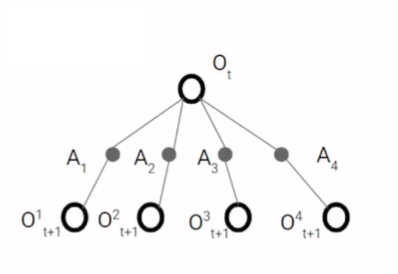
\includegraphics[width=0.6\linewidth,keepaspectratio]{rl18}
\end{center}


{\tiny (Ref: But what is Reinforcement Learning? | Reinforcement Learning Part-1 - Rajtilak Pal (M. Tech in AI, IIT Ropar))}

\end{frame}

%%%%%%%%%%%%%%%%%%%%%%%%%%%%%%%%%%%%%%%%%%%%%%%%%%%%%%%%%%%%%%%%%%%%%%%%%%%%%%%%%%
\begin{frame}[fragile]\frametitle{Path Generation}

Policy function decides which of these Actions are most promising. Here $A_1, A_3$ are.

\begin{center}
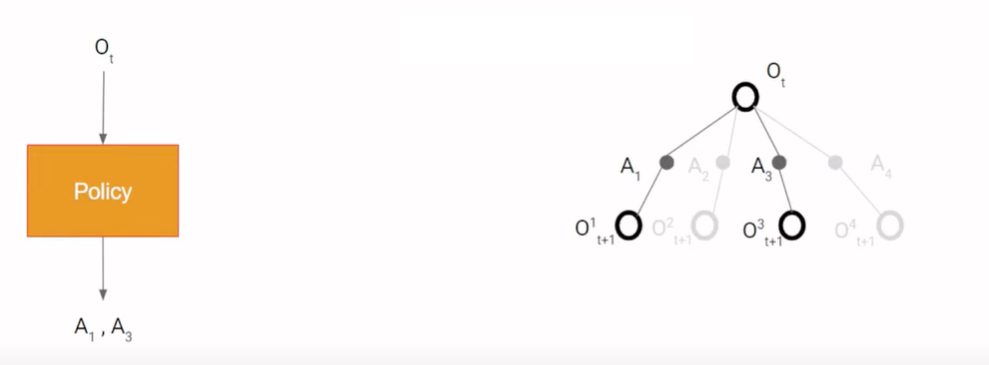
\includegraphics[width=\linewidth,keepaspectratio]{rl19}
\end{center}


{\tiny (Ref: But what is Reinforcement Learning? | Reinforcement Learning Part-1 - Rajtilak Pal (M. Tech in AI, IIT Ropar))}

\end{frame}

%%%%%%%%%%%%%%%%%%%%%%%%%%%%%%%%%%%%%%%%%%%%%%%%%%%%%%%%%%%%%%%%%%%%%%%%%%%%%%%%%%
\begin{frame}[fragile]\frametitle{Path Generation}

Follow same procedure till end. 

\begin{center}
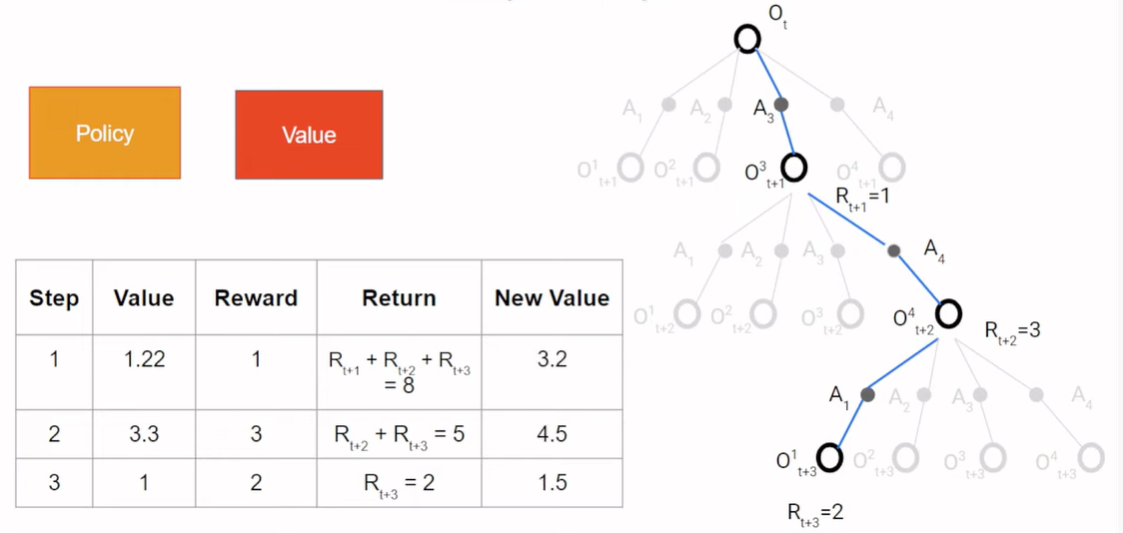
\includegraphics[width=\linewidth,keepaspectratio]{rl20}
\end{center}


{\tiny (Ref: But what is Reinforcement Learning? | Reinforcement Learning Part-1 - Rajtilak Pal (M. Tech in AI, IIT Ropar))}

\end{frame}


%%%%%%%%%%%%%%%%%%%%%%%%%%%%%%%%%%%%%%%%%%%%%%%%%%%%%%%%%%%%%%%%%%%%%%%%%%%%%%%%%%
\begin{frame}[fragile]\frametitle{Path Generation}

Once it has all rewards, then it adjust the values (Q-Learning?).

\begin{center}
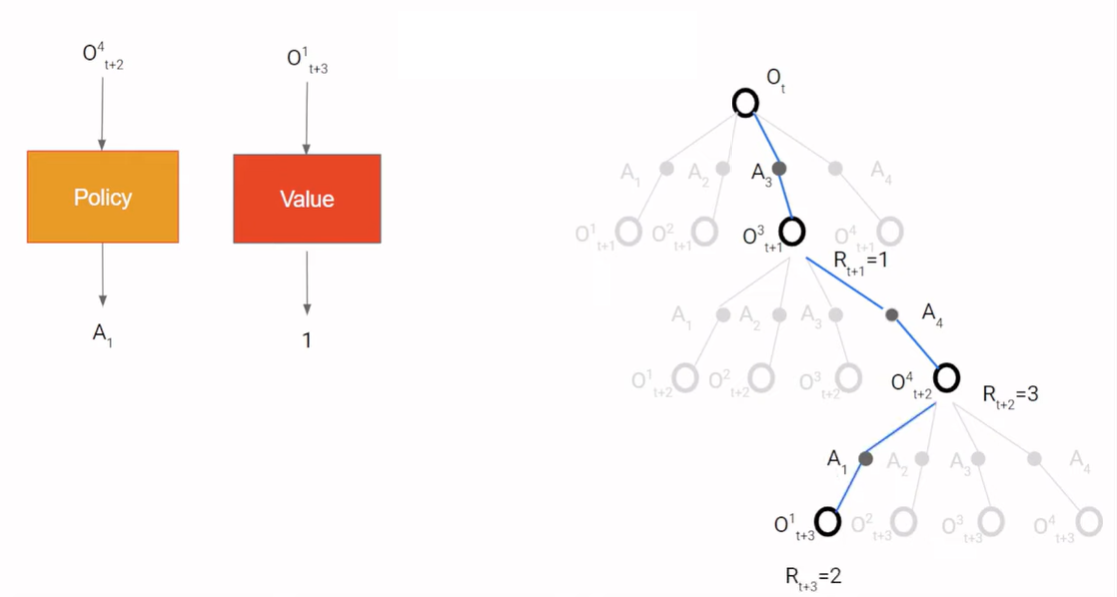
\includegraphics[width=\linewidth,keepaspectratio]{rl21}
\end{center}


{\tiny (Ref: But what is Reinforcement Learning? | Reinforcement Learning Part-1 - Rajtilak Pal (M. Tech in AI, IIT Ropar))}

\end{frame}

%%%%%%%%%%%%%%%%%%%%%%%%%%%%%%%%%%%%%%%%%%%%%%%%%%%%%%%%%%%%%%%%%%%%%%%%%%%%%%%%%%
\begin{frame}[fragile]\frametitle{State Value Function}

\begin{itemize}
\item State Value Functions $v_{\pi}$ gives the value of a State $s$ under given Policy $\pi$
\item How good is a State for the Agent following the Policy $\pi$
\end{itemize}

$v_{\pi}(s) = E_{\pi}[G_t | S_t = s] = E_{\pi}[\sum_{k=0}^{\infty}\gamma^kR_{t+k+1}|S_t=s]$

\end{frame}

%%%%%%%%%%%%%%%%%%%%%%%%%%%%%%%%%%%%%%%%%%%%%%%%%%%%%%%%%%%%%%%%%%%%%%%%%%%%%%%%%%
\begin{frame}[fragile]\frametitle{Action Value Function, Q Function}

\begin{itemize}
\item Method to estimate value of an Action, and then selecting among pool of such available Actions.
\item True (actual) value of Action $a$ is $Q^*(a)$ and the estimated value after $t$ time-steps is $Q_t(a)$.
\item True value of an Action is the mean reward given that the Action is selected. Ratio of sum of rewards when $a$ taken prior to $t$, to number of tomes a taken prior to $t$. $Q_t(a) = = \frac{\sum_{i=1}^{t-1} R_i}{t-1}$
\item Action Value Functions $q_{\pi}$ gives the value of a State-Action pair $(s,a)$ 
\item Q - quality of taking a given Action in a given State to determine best Policy $\pi$ for the Agent.
\item For small problems, Q values are in form of a table, States as rows and Actions as columns.
\end{itemize}

\end{frame}


\section[Opt]{Learning Optimum Policy}

%%%%%%%%%%%%%%%%%%%%%%%%%%%%%%%%%%%%%%%%%%%%%%%%%%%%%%%%%%%%%%%%%%%%%%%%%%%%%%%%%%
\begin{frame}[fragile]\frametitle{}
\begin{center}
{\Large Learning Optimum Policy}
\end{center}
\end{frame}


%%%%%%%%%%%%%%%%%%%%%%%%%%%%%%%%%%%%%%%%%%%%%%%%%%%%%%%%%%%%%%%%%%%%%%%%%%%%%%%%%%
\begin{frame}[fragile]\frametitle{Optimal Policy}

$\pi \geq \pi' \iff v_{\pi}(s) \geq {v'}_{\pi}(s) \forall s \in S$

\begin{itemize}
\item A Policy is measured based on State Value function
\item So, whichever Policy has State Value function better at the given State, is considered better
\end{itemize}

\end{frame}

%%%%%%%%%%%%%%%%%%%%%%%%%%%%%%%%%%%%%%%%%%%%%%%%%%%%%%%%%%%%%%%%%%%%%%%%%%%%%%%%%%
\begin{frame}[fragile]\frametitle{Optimal State Value Function}

$v_{*}(s) = max_{\pi} v_{\pi}(s) \forall s \in S$

$v_{*}$ gives the largest expected return achievable by any Policy $\pi$ for each State.

\end{frame}

%%%%%%%%%%%%%%%%%%%%%%%%%%%%%%%%%%%%%%%%%%%%%%%%%%%%%%%%%%%%%%%%%%%%%%%%%%%%%%%%%%
\begin{frame}[fragile]\frametitle{Optimal Action Value Function}

$q_{*}(s,a) = max_{\pi} q_{\pi}(s,a) \forall s \in S, a \in A(s)$

$q_{*}$ gives the largest expected return achievable by any Policy $\pi$ for each State-Action pair.

\end{frame}

%%%%%%%%%%%%%%%%%%%%%%%%%%%%%%%%%%%%%%%%%%%%%%%%%%%%%%%%%%%%%%%%%%%%%%%%%%%%%%%%%%
\begin{frame}[fragile]\frametitle{Bellman Optimality Equation for Action Value Function}

\begin{itemize}
\item According to Bellman Optimality Equation, $q_{*}$ must satisfy,

$q_{*}(s,a) = E[R{t+1} + \gamma max_{a'} q_{*}(s',a')]$

\item Optimal Policy is found by applying iterative RL algorithms to find the Action that maximizes $q_*$ for each State.

\item Calculating $q_*$ for each state is very cumbersome if the State space is very large. Some approximation is applied like Dynamic Programming, Monte Carlo Method and Temporal Difference.
\end{itemize}

\end{frame}

%%%%%%%%%%%%%%%%%%%%%%%%%%%%%%%%%%%%%%%%%%%%%%%%%%%%%%%%%%%%%%%%%%%%%%%%%%%%%%%%%%
\begin{frame}[fragile]\frametitle{So, formally, RL}

\begin{center}
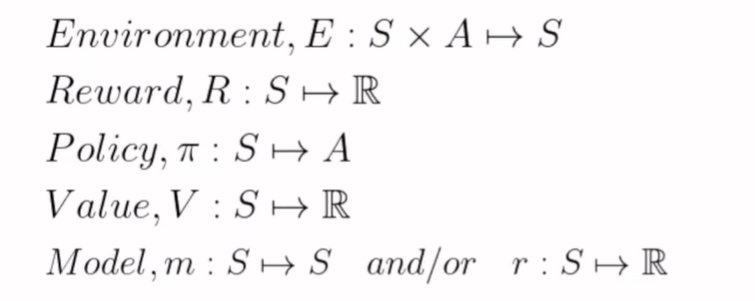
\includegraphics[width=0.6\linewidth,keepaspectratio]{rl23}
\end{center}

{\tiny (Ref: But what is Reinforcement Learning? | Reinforcement Learning Part-1 - Rajtilak Pal (M. Tech in AI, IIT Ropar))}
\end{frame}


\section[Q-Learn]{Q-Learning Algorithm}

%%%%%%%%%%%%%%%%%%%%%%%%%%%%%%%%%%%%%%%%%%%%%%%%%%%%%%%%%%%%%%%%%%%%%%%%%%%%%%%%%%
\begin{frame}[fragile]\frametitle{}
\begin{center}
{\Large Q-Learning Algorithm}
\end{center}
\end{frame}

%%%%%%%%%%%%%%%%%%%%%%%%%%%%%%%%%%%%%%%%%%%%%%%%%%%%%%%%%%%%%%%%%%%%%%%%%%%%%%%%%%
\begin{frame}[fragile]\frametitle{Goal}

Q-Learning is:

\begin{itemize}
\item Algorithm to solve Optimal Policy in a MDP
\item Learns the optimal Q-value for each State-Action pair
\item Maximizes the expected Value of the total Reward over all steps.
\end{itemize}

\end{frame}

%%%%%%%%%%%%%%%%%%%%%%%%%%%%%%%%%%%%%%%%%%%%%%%%%%%%%%%%%%%%%%%%%%%%%%%%%%%%%%%%%%
\begin{frame}[fragile]\frametitle{Approaches}
\begin{center}
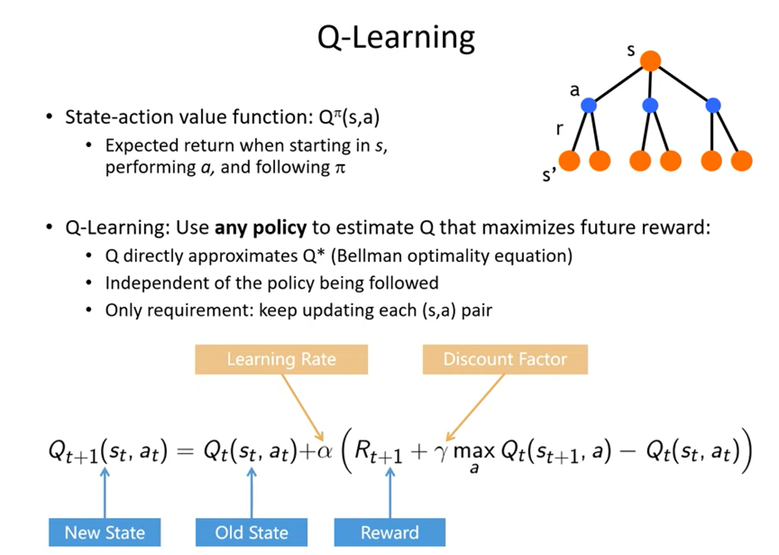
\includegraphics[width=0.8\linewidth,keepaspectratio]{rl27}
\end{center}

{\tiny (Ref: Deep Learning - MIT 2019)}

\end{frame}

%%%%%%%%%%%%%%%%%%%%%%%%%%%%%%%%%%%%%%%%%%%%%%%%%%%%%%%%%%%%%%%%%%%%%%%%%%%%%%%%%%
\begin{frame}[fragile]\frametitle{Value Iteration}

\begin{itemize}
\item Bellman Optimality Equation is:

$q_{*}(s,a) = E[R{t+1} + \gamma max_{a'} q_{*}(s',a')]$


\item The Q-Learning algorithm iteratively updates the Q-values for each State-Action pair using the Bellman Equation until the Q-Function coverages to the optimal Q-function $q_*$
\end{itemize}

\end{frame}

%%%%%%%%%%%%%%%%%%%%%%%%%%%%%%%%%%%%%%%%%%%%%%%%%%%%%%%%%%%%%%%%%%%%%%%%%%%%%%%%%%
\begin{frame}[fragile]\frametitle{Foraging Agent}

\begin{center}
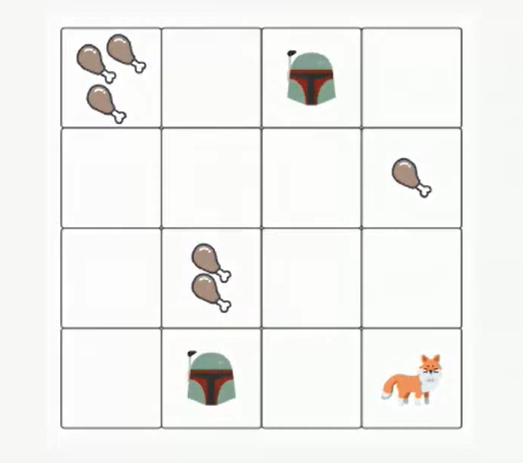
\includegraphics[width=0.5\linewidth,keepaspectratio]{rl3}
\end{center}

\begin{itemize}
\item Fox wants to get meat but avoid hunters.
\item The whole grid is an Environment, boxes are States and the fox is the agent. Reward is meat/hunter. Actions are up-down-right-left movements.
\end{itemize}

\end{frame}

%%%%%%%%%%%%%%%%%%%%%%%%%%%%%%%%%%%%%%%%%%%%%%%%%%%%%%%%%%%%%%%%%%%%%%%%%%%%%%%%%%
\begin{frame}[fragile]\frametitle{Rewards}

\begin{columns}
\begin{column}{0.5\textwidth}

\begin{center}
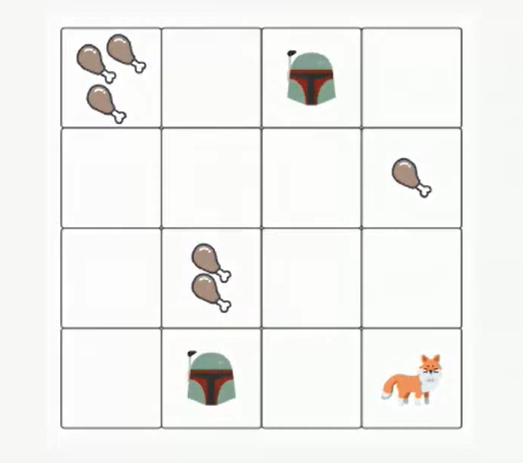
\includegraphics[width=\linewidth,keepaspectratio]{rl3}
\end{center}

\end{column}
\begin{column}{0.5\textwidth}  %%<--- here

\begin{itemize}
\item Empty : $-1$ as movement requires some effort
\item One meat : $+1$
\item Two meat : $+2$
\item Three meat : $+3$
\item Hunter : $-5$ game over
\item Maximum reward: game over (ie $+6$)
\end{itemize}

\end{column}
\end{columns}

\end{frame}

%%%%%%%%%%%%%%%%%%%%%%%%%%%%%%%%%%%%%%%%%%%%%%%%%%%%%%%%%%%%%%%%%%%%%%%%%%%%%%%%%%
\begin{frame}[fragile]\frametitle{Q-Value Table}

\begin{columns}
\begin{column}{0.5\textwidth}
Initialized to 0s at the start. Empty boxes are numbered from top and then to right and so on.

\end{column}
\begin{column}{0.5\textwidth}  %%<--- here
\begin{center}
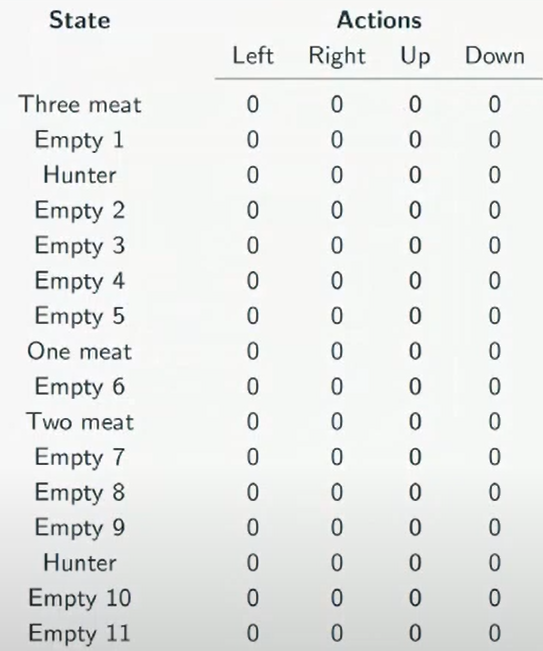
\includegraphics[width=\linewidth,keepaspectratio]{rl4}
\end{center}
\end{column}
\end{columns}
\end{frame}

%%%%%%%%%%%%%%%%%%%%%%%%%%%%%%%%%%%%%%%%%%%%%%%%%%%%%%%%%%%%%%%%%%%%%%%%%%%%%%%%%%
\begin{frame}[fragile]\frametitle{Epsilon Greedy Strategy}


\begin{itemize}
\item Exploration rate $\epsilon$, 1 to start with. Meaning the Agent with Explore (random walk) 100\% of time.
\item At the start of each new episode $\epsilon$ will decay-reduce, then the Agent will become GREEDY and start Exploiting.
\item In the algorithm, generate random number $r$ between 0 and 1.
\item if $r > \epsilon$ the Agent will Exploit (meaning, use past experience based formulation to get the next Action), else it will Explore (meaning, the next Action proposed would be randomly selected from the given set of Actions)
\end{itemize}

\end{frame}


%%%%%%%%%%%%%%%%%%%%%%%%%%%%%%%%%%%%%%%%%%%%%%%%%%%%%%%%%%%%%%%%%%%%%%%%%%%%%%%%%%
\begin{frame}[fragile]\frametitle{Move}

\begin{itemize}
\item Fox moves up (say, via random). So, reward is $-1$. 
\item To update the Q-value for the Action of Moving Up taken from the previous State, using Bellman Equation and applying Learning rate $\alpha$ (to control the speed, just like in Gradient Descent).
\item At start, initial q value was 0 and with $\alpha = 0.7, \gamma = 0.99$

\item 

$q^{new}(s,a) = (1 - \alpha)\underbrace{q(s,a)}^\text{old value} + \alpha \overbrace{(R_{t+1} + \gamma max_{a'} q(s',a'))}^\text{learning rate} = (1-0.7)(0) + 0.7(-1 + 0.99(max_{a'} q(s',a')))$ 
\item where, $max_{a'} q(s',a') = max(q(empty8,left), q(empty8, up), q(empty8,down)) = max(-1,1,-1) = 1$ where 'empty8' is the moved position. $+1$ because there is 1 meat there if moves further up.
\item $= (1-0.7)(0) + 0.7(-1, 0.99(1)) = 0 + 0.7(-0.01) = -0.007$
\item Update the Q table and repeat till converges to Optimal Policy (how?)
\end{itemize}

\end{frame}

%%%%%%%%%%%%%%%%%%%%%%%%%%%%%%%%%%%%%%%%%%%%%%%%%%%%%%%%%%%%%%%%%%%%%%%%%%%%%%%%%%
\begin{frame}[fragile]\frametitle{Problems}
\begin{center}
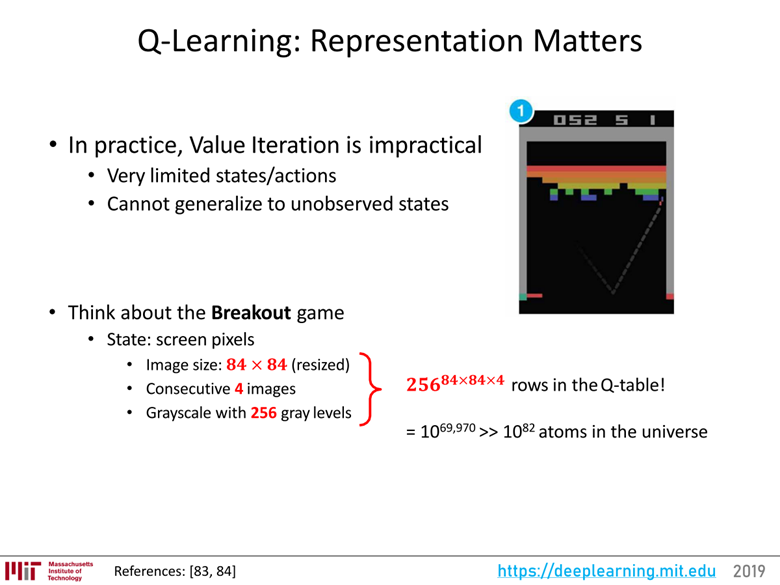
\includegraphics[width=0.7\linewidth,keepaspectratio]{rl28}
\end{center}

{\tiny (Ref: Deep Learning - MIT 2019)}

Solution for this very High Dimensionality problem is Neural Networks. They approximate the Q-function.

\end{frame}


%%%%%%%%%%%%%%%%%%%%%%%%%%%%%%%%%%%%%%%%%%%%%%%%%%%%%%%%%%%%%%%%%%%%%%%%%%%%%%%%%%
\begin{frame}[fragile]\frametitle{Deep Q Learning}

\begin{itemize}
\item Instead of Q table, if neural network is employed which takes a State as input and gives approximate Q values for different actions, then thats Deep Q learning
\item Useful especially if there are too many states and complexity.
\end{itemize}

\begin{center}
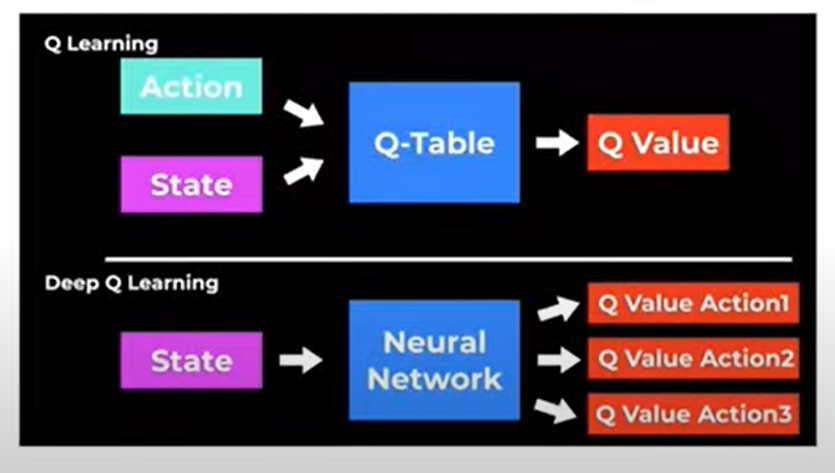
\includegraphics[width=0.6\linewidth,keepaspectratio]{rl10}
\end{center}

{\tiny (Ref: Deep Q Network, a deep reinforcement learning approach - Nitin Mukesh)}
\end{frame}


%%%%%%%%%%%%%%%%%%%%%%%%%%%%%%%%%%%%%%%%%%%%%%%%%%%%%%%%%%%%%%%%%%%%%%%%%%%%%%%%%%
\begin{frame}[fragile]\frametitle{Deep Q Learning}

Some times Experience Replay or Action Replay memory is used, where one calculation ie $(s_t,a_t,r_t,s_{t+1})$ tuple is stored in the memory. All such entries forms a training data, which can train the neural network.

\begin{center}
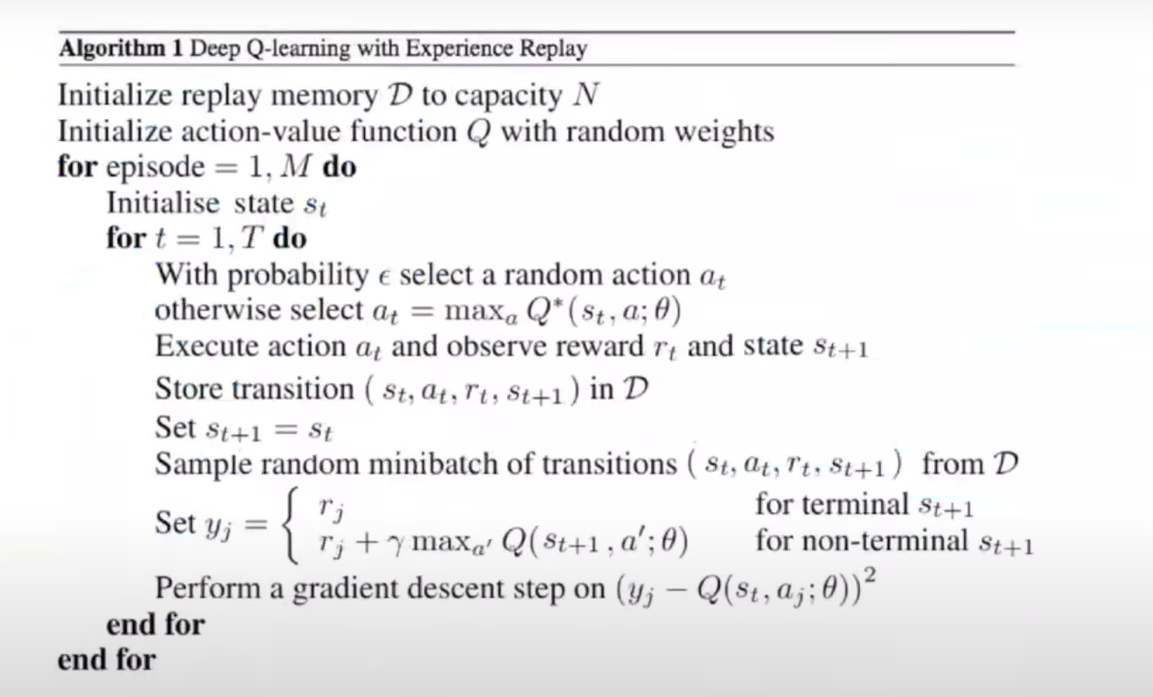
\includegraphics[width=0.8\linewidth,keepaspectratio]{rl11}
\end{center}

{\tiny (Ref: Deep Q Network, a deep reinforcement learning approach - Nitin Mukesh)}
\end{frame}

%%%%%%%%%%%%%%%%%%%%%%%%%%%%%%%%%%%%%%%%%%%%%%%%%%%%%%%%%%%%%%%%%%%%%%%%%%%%%%%%%%
\begin{frame}[fragile]\frametitle{Deep Q-Network}
\begin{center}
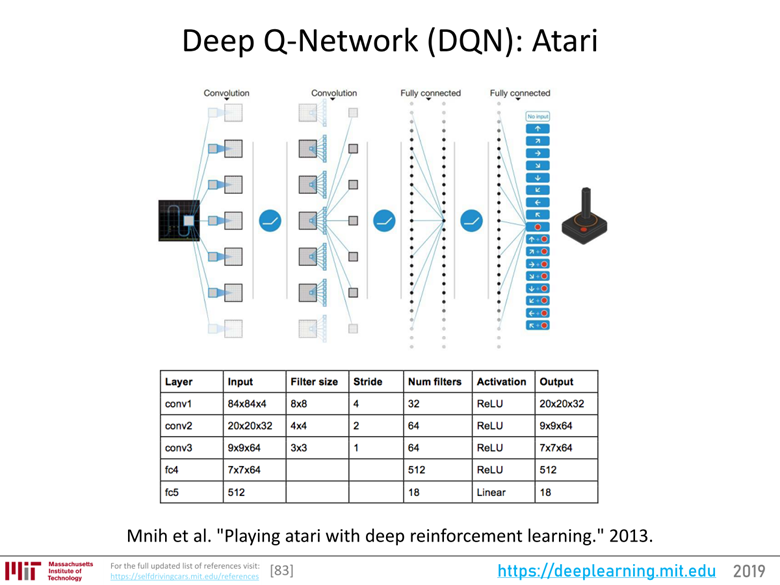
\includegraphics[width=0.8\linewidth,keepaspectratio]{rl29}
\end{center}

{\tiny (Ref: Deep Learning - MIT 2019)}


\end{frame}


%%%%%%%%%%%%%%%%%%%%%%%%%%%%%%%%%%%%%%%%%%%%%%%%%%%%%%%%%%%%%%%%%%%%%%%%%%%%%%%%%%
\begin{frame}[fragile]\frametitle{DQN Tricks}

\begin{itemize}
\item Experience Replay: Stores experiences (actions, state transitions, and rewards) and creates mini batches from them for the training process
\item Fixed Target Network: Error calculation includes the target function depends on network parameters and thus changes quickly. Updating it only every 1,000 steps increase stability of training process.
\end{itemize}

Policy Gradient (PG)
\begin{itemize}
\item DQN (off-policy): Approximate Q and infer optimal policy
\item PG (on-policy): Directly optimize policy space
\end{itemize}

\end{frame}



\section[Example]{Implementation}

%%%%%%%%%%%%%%%%%%%%%%%%%%%%%%%%%%%%%%%%%%%%%%%%%%%%%%%%%%%%%%%%%%%%%%%%%%%%%%%%%%
\begin{frame}[fragile]\frametitle{}
\begin{center}
{\Large Implementation}
\end{center}
\end{frame}

%%%%%%%%%%%%%%%%%%%%%%%%%%%%%%%%%%%%%%%%%%%%%%%%%%%%%%%%%%%%%%%%%%%%%%%%%%%%%%%%%%
\begin{frame}[fragile]\frametitle{How to learn Policy?}

\begin{center}
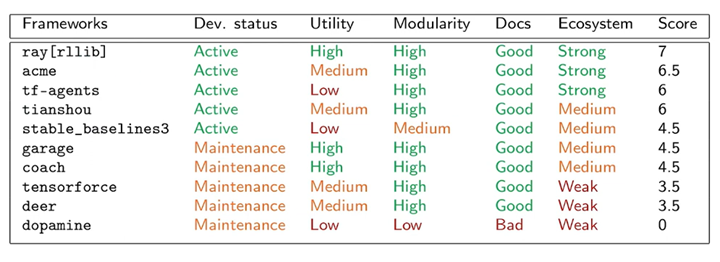
\includegraphics[width=0.8\linewidth,keepaspectratio]{rl51}
\end{center}

{\tiny (Ref: Which Reinforcement Learning Framework is the Best?)}

‘rlib’ is part of `ray’ project.

\end{frame}


%%%%%%%%%%%%%%%%%%%%%%%%%%%%%%%%%%%%%%%%%%%%%%%%%%%%%%%%%%%%%%%%%%%%%%%%%%%%%%%%%%
\begin{frame}[fragile]\frametitle{Reinforcement Learning Work-flow}

\begin{itemize}
\item Create the Environment
\item Define the reward
\item Create the agent
\item Train and validate the agent
\item Deploy the policy
\end{itemize}

\begin{center}
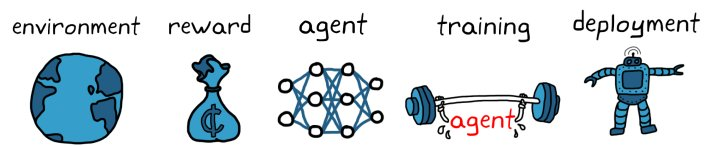
\includegraphics[width=0.8\linewidth,keepaspectratio]{rl6}

{\tiny (Ref: Reinforcement Learning Work-flow - KDNuggets)} 
\end{center}

\end{frame}



%%%%%%%%%%%%%%%%%%%%%%%%%%%%%%%%%%%%%%%%%%%%%%%%%%%%%%%%%%%%%%%%%%%%%%%%%%%%%%%%%%
\begin{frame}[fragile]\frametitle{Problem: Frozen Lake Game}


You need to walk from starting State ($S$) to the goal State ($G$) by walking on frozen tiles ($F$) only and avoiding holes ($H$).


\begin{center}
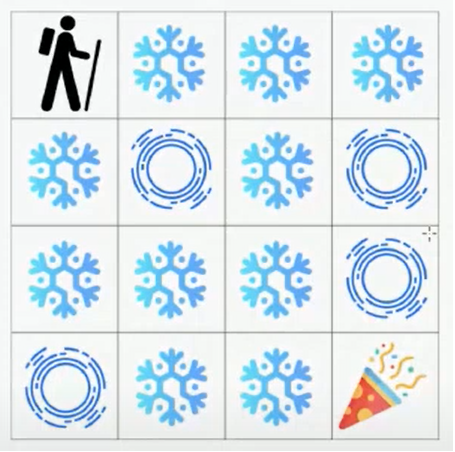
\includegraphics[width=0.4\linewidth,keepaspectratio]{rl5}
\end{center}

\end{frame}

%%%%%%%%%%%%%%%%%%%%%%%%%%%%%%%%%%%%%%%%%%%%%%%%%%%%%%%%%%%%%%%%%%%%%%%%%%%%%%%%%%
\begin{frame}[fragile]\frametitle{Code}

\begin{lstlisting}
from tf_agents.environments import suite_gym

# create the environment
env = suite_gym("FrozenLake-v0")

# create Q-table
action_size = env.action_space.n
state_size = env.state_space.n
qtable = np.zeros((state_size,action_space))

# parameters
total_episodes = 30000
learning_rate = 0.1
max_steps = 100 # per episode
gamma = 0.99
epsilon = 1.0
max_epsilon = 1.0
min_epsilon = 0.01
decay_rate = 0.01

\end{lstlisting}

\end{frame}


%%%%%%%%%%%%%%%%%%%%%%%%%%%%%%%%%%%%%%%%%%%%%%%%%%%%%%%%%%%%%%%%%%%%%%%%%%%%%%%%%%
\begin{frame}[fragile]\frametitle{Training}

\begin{lstlisting}
rewards = []
for episode in range(total_episodes):
	state = env.reset()
	step = 0
	done = False
	total_rewards = 0
	for step in range(max_steps):
		exp_exp_tradeoff = random.uniform(0,1)
		if exp_exp_tradeoff > epsilon: # exploitation
			action = np.argmax(qtable[state,:])
		else: # random, exploration
			action = env.action_space.sample()
		new_state, reward, done, info = env.step(action)
		qtable[state,action] = qtable[state,action] + 
		learning_rate * (reward + gamma * np.max(qtable[new_state,:]) 
		- qtable[state,action]) 
		total_rewards += reward
		state = new_state
		if done == True:
			break
	epsilon = min_epsilon + (max_epsilon - min_epsilon)*np.exp(-decay_rate*episode)
	rewards.append(total_rewards)

\end{lstlisting}

\end{frame}

%%%%%%%%%%%%%%%%%%%%%%%%%%%%%%%%%%%%%%%%%%%%%%%%%%%%%%%%%%%%%%%%%%%%%%%%%%%%%%%%%%
\begin{frame}[fragile]\frametitle{Testing}

\begin{lstlisting}
env.reset()
for episode in range(5):
	state = env.reset()
	step = 0
	done = False
	for step in range(max_steps):
		action = np.argmax(qtable[state,:])
		new_state, reward, done, info = env.step(action)
		if done == True:
			env.render()
			break
		state = new_state
env.close()
\end{lstlisting}

\end{frame}



\section[End]{The End}

%%%%%%%%%%%%%%%%%%%%%%%%%%%%%%%%%%%%%%%%%%%%%%%%%%%%%%%%%%%%%%%%%%%%%%%%%%%%%%%%%%
\begin{frame}[fragile]\frametitle{}
\begin{center}
{\Large Conclusion}
\end{center}
\end{frame}


%%%%%%%%%%%%%%%%%%%%%%%%%%%%%%%%%%%%%%%%%%%%%%%%%%%%%%%%%%%%%%%%%%%%%%%%%%%%%%%%%%
\begin{frame}[fragile]\frametitle{Conclusion}

\begin{itemize}
\item RL helps us to discover which action could yield the highest reward for a longer time. 
\item Realistic environments can have partial observability and be non-stationary as well. 
\item It isn’t very useful to apply when you have hands-on enough data to solve the problem using supervised learning. \item The main challenge of this method is that parameters could affect the speed of the learning.
\end{itemize}



\end{frame}

%%%%%%%%%%%%%%%%%%%%%%%%%%%%%%%%%%%%%%%%%%%%%%%%%%%%%%%%%%%%%%%%%%%%%%%%%%%%%%%%%%
\begin{frame}[fragile]\frametitle{How to get started?}

\begin{itemize}
\item Reinforcement Learning-An Introduction, a book by the father of Reinforcement Learning- Richard Sutton and his doctoral advisor Andrew Barto. An online draft available.
\item Course by David Silver including video lectures.
\item Technical tutorial by Pieter Abbeel and John Schulman (Open AI/ Berkeley AI Research Lab).
\item "Deep Reinforcement Learning: Pong from Pixels" - Andrej Karpathy blog
\end{itemize}

\end{frame}


%%%%%%%%%%%%%%%%%%%%%%%%%%%%%%%%%%%%%%%%%%%%%%%%%%%%%%%%%%%%%%%%%%%%%%%%%%%%%%%%%%
\begin{frame}\frametitle{References}
\begin{itemize}
\item Learning in Random Environments - Ekaba Bisong
\item Reinforcement Learning : Playing to Win - Shweta Bhatt
\item Reinforcement Learning 101 - Shweta Bhatt
\item Deep Q Network, a deep reinforcement learning approach - Nitin Mukesh
\item Introduction to Reinforcement Learning for Beginners -  Prathima Kadari, Analytics Vidhya
\end{itemize}
\end{frame}